\begin{figure}[h]
	\centering    
    \begin{tikzpicture}
    \node[inner sep=0pt] (pic) at (0,0)
    {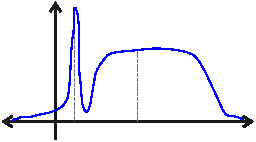
\includegraphics[width=10cm]{pictures/picture_2_1.pdf}};
    \draw [color=black](-2.5,-2) node[anchor=north west] {$ \widehat{\t}_{\text{MLE}} $};
    \draw [color=black](0.2,-2) node[anchor=north west] {$ \widehat{\t}_{\text{B}} $};
    \draw [color=blue](2.8,1.2) node[anchor=north west] {$ \pi(\t|\textbf{x}) $};
    \end{tikzpicture}
	\caption{Možný tvar aposteriorní hustoty pravděpodobnosti. Demonstrace skutečnosti, že MLE odhad nemusí být vždy nejlepší.}
\end{figure}